\documentclass{article}

\usepackage{graphicx}
\usepackage{tikz}
\usepackage{tikzsymbols}
\usetikzlibrary{calc,patterns,shapes.geometric}
\pagestyle{empty}
\usepackage[margin=0pt]{geometry}
\geometry{papersize={14in,12in}}

\def\centerarc[#1](#2)(#3:#4:#5){\draw[#1] ($(#2)+({#5*cos(#3)},{#5*sin(#3)})$) arc (#3:#4:#5);}

\begin{document}
	\begin{figure}
		\centering
		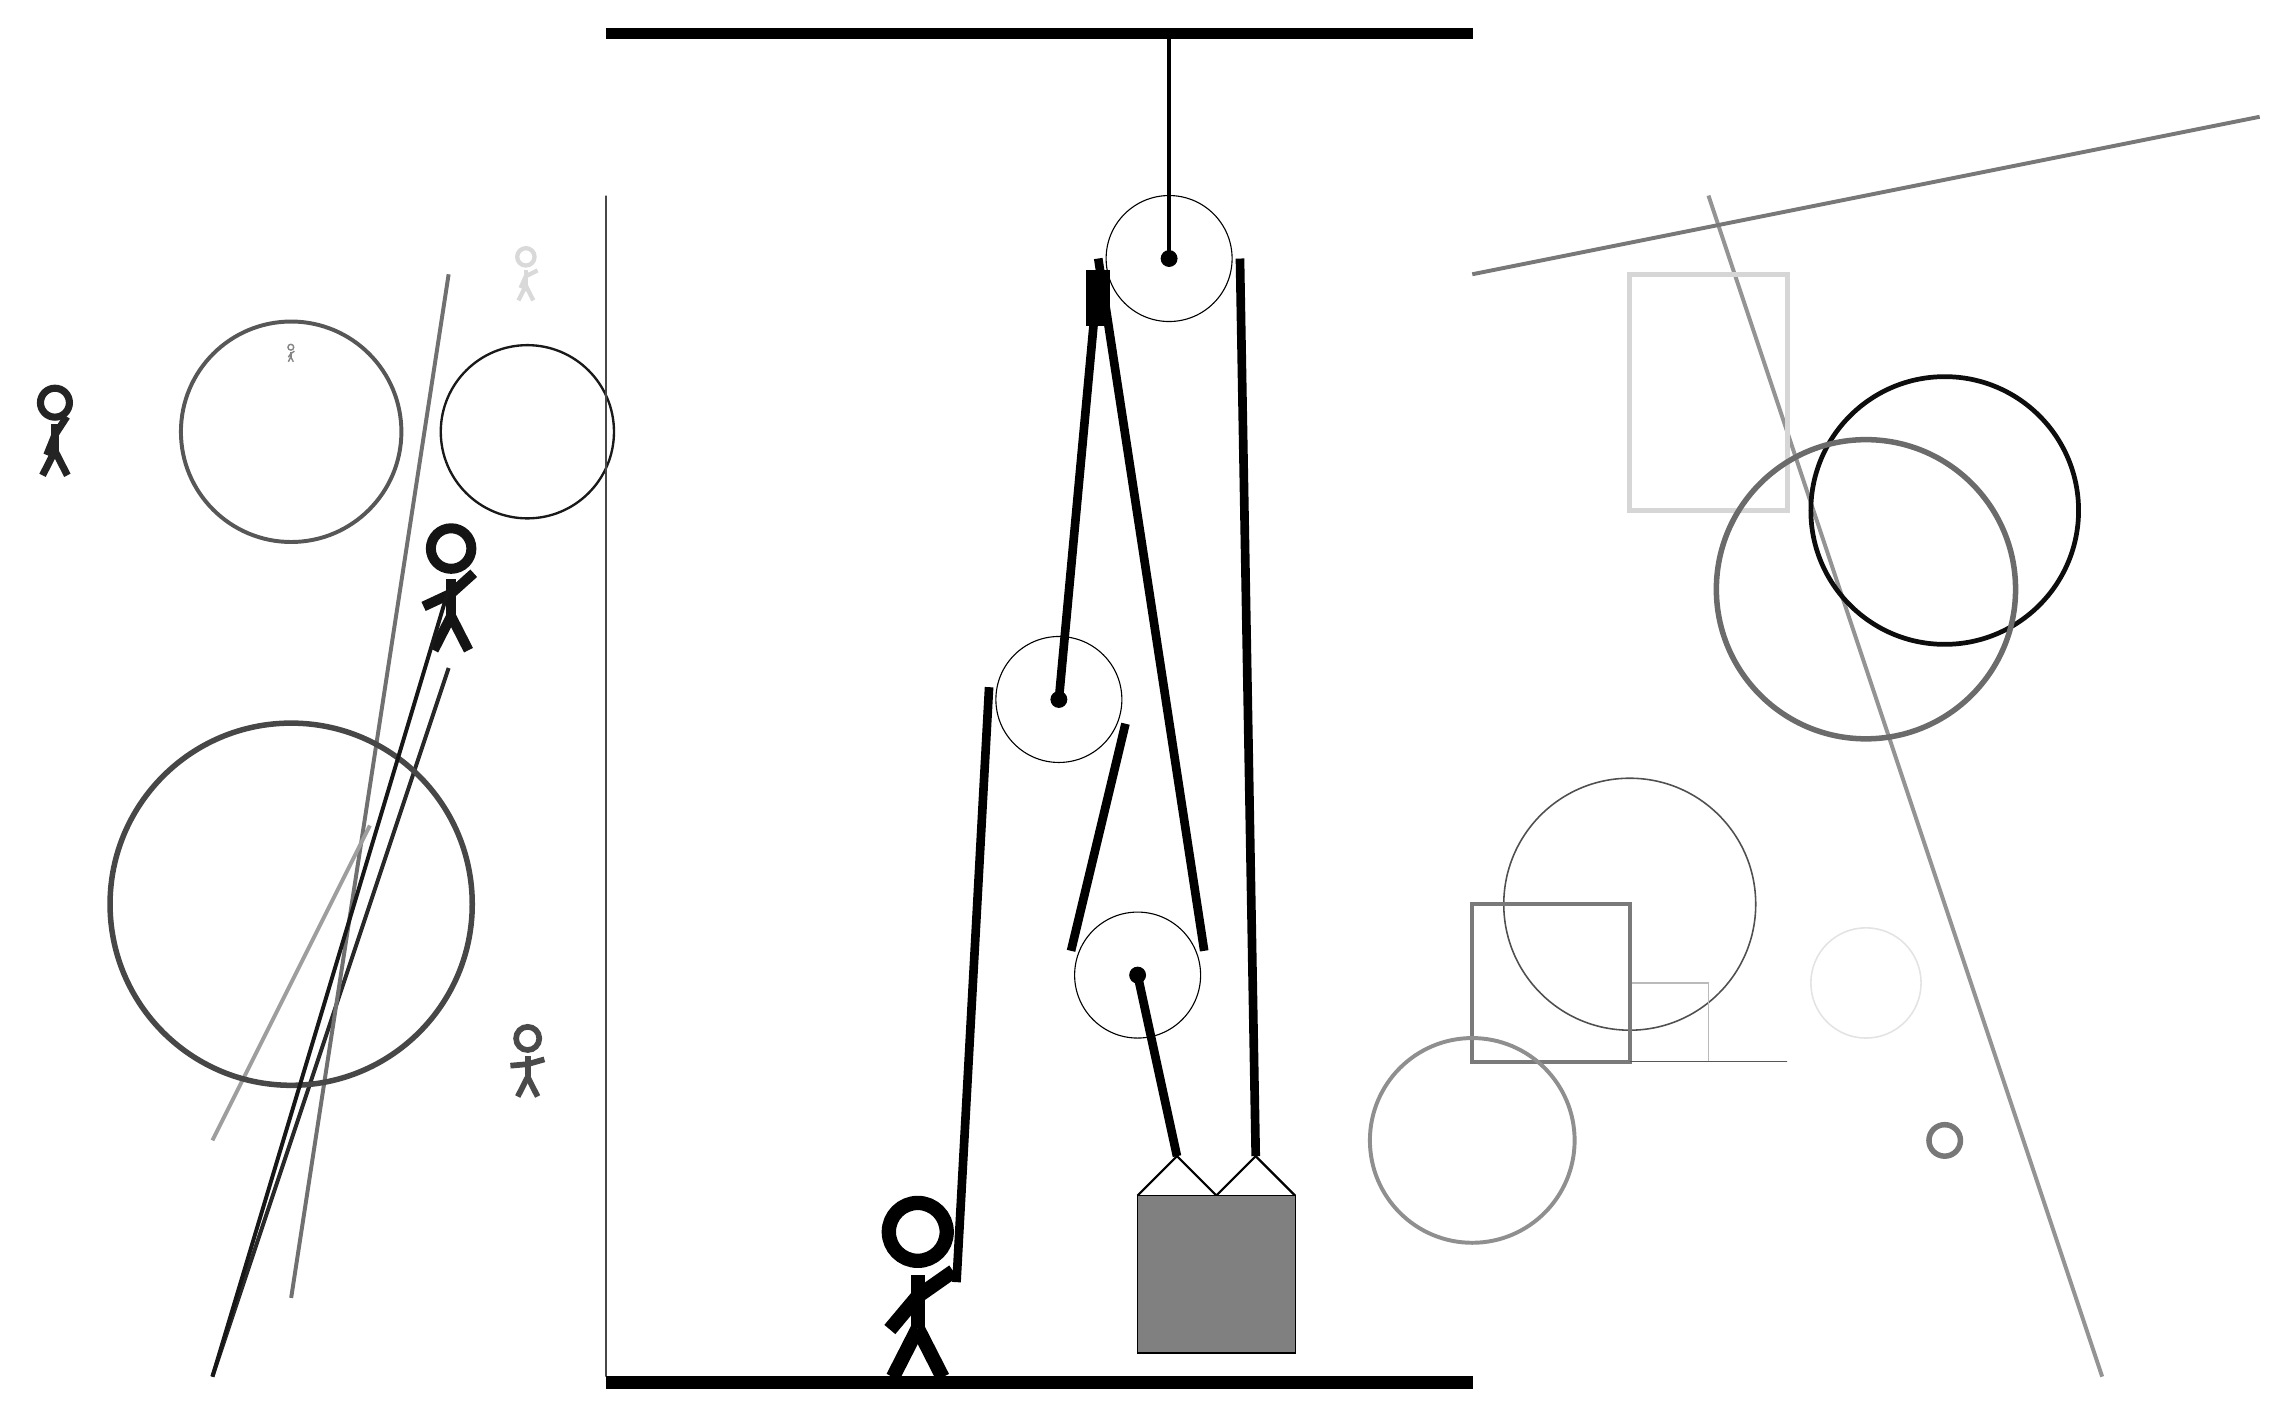
\begin{tikzpicture}
			%%%%% START %%%%%
			
			\draw[fill=black] (-6, 14) rectangle (5, 14.125);
			
			\draw (-0.25, 5.6) circle (0.8);
			\draw[fill=black] (-0.25, 5.6) circle (0.1);
			
			\draw (0.75, 2.1) circle (0.8);
			\draw[fill=black] (0.75, 2.1) circle (0.1);
			
			\draw (1.15, 11.2) circle (0.8);
			\draw[fill=black] (1.15, 11.2) circle (0.1);
			\draw[very thick] (1.15, 11.2) -- (1.15, 14);
			
			\draw[thick]  (0.75, -0.7) -- (1.25, -0.2) -- (1.75, -0.7) -- (2.25, -0.2) -- (2.75, -0.7);
			\draw[fill=black!50] (0.75, -0.7) rectangle (2.75, -2.7);
			
			\draw[line width=1.1mm] (-0.25, 5.6) -- (0.25, 11.0);
			\draw[line width=1.1mm, fill=black](0.15, 10.4) rectangle (0.35, 11.0);
			\draw[line width=1.1mm] (-1.55, -1.8) -- (-1.1363, 5.7562);
			\centerarc[line width=1.1mm](-0.25, 5.6)(-20:170:0.9);
			\draw[line width=1.1mm] (0.5957, 5.2922) -- (-0.0957, 2.4078);
			\centerarc[line width=1.1mm](0.75, 2.1)(160:380:0.9);
			\draw[line width=1.1mm] (1.5957, 2.4078) -- (0.25, 11.2);
			\draw[line width=1.1mm](0.75, 2.1) -- (1.25, -0.2);
			\centerarc[line width=1.1mm](1.15, 11.2)(0:180:0.9);
			\draw[line width=1.1mm] (2.05, 11.2) -- (2.25, -0.2);
			
			\node at (-2, -1.9) {\Strichmaxerl[10][50][35]};
			
			\node[line width=0.5mm, color=black!92] at (-8, 7) {\Strichmaxerl[7][25][42]};
			
			\draw[line width=0.5mm, color=black!42](8, 12) -- (13, -3);
			\draw [line width=0.6mm, color=black!95](11, 8) circle (1.7);
			\draw[line width=0.5mm, color=black!84](-8, 6) -- (-11, -3);
			\draw [line width=0.3mm, color=black!90](-7, 9) circle (1.1);
			\draw[line width=0.5mm, color=black!56](-8, 11) -- (-10, -2);
			\draw[line width=0.5mm, color=black!53](5, 11) -- (15, 13);
			
			\draw [line width=0.2mm, color=black!69](7, 3) circle (1.6);
			\draw[line width=0.2mm, color=black!72] (-6, 12) rectangle (-6, -3);
			\draw[line width=0.5mm, color=black!38](-9, 4) -- (-11, 0);
			\node[line width=0.3mm, color=black!48] at (-10, 10) {\Strichmaxerl[1][55][35]};
			\draw[line width=0.2mm, color=black!27] (7, 1) rectangle (8, 2);
			\draw [line width=0.7mm, color=black!72](-10, 3) circle (2.3);
			
			\node[line width=0.6mm, color=black!15] at (-7, 11) {\Strichmaxerl[3][66][26]};
			\draw[line width=0.5mm, color=black!52] (7, 3) rectangle (5, 1);
			\draw [line width=0.5mm, color=black!66](-10, 9) circle (1.4);
			
			\draw[line width=0.2mm, color=black!66] (7, 1) rectangle (9, 1);
			
			\draw [line width=0.2mm, color=black!11](10, 2) circle (0.7);
			\node[line width=0.6mm, color=black!71] at (-7, 1) {\Strichmaxerl[4][5][16]};
			
			\draw [line width=0.5mm, color=black!44](5, 0) circle (1.3);
			\draw [line width=0.7mm, color=black!53](11, 0) circle (0.2);
			\draw[line width=0.6mm, color=black!16] (7, 8) rectangle (9, 11);
			\draw[line width=0.5mm, color=black!91](-11, -3) -- (-8, 7);
			\node[line width=0.4mm, color=black!86] at (-13, 9) {\Strichmaxerl[5][68][57]};
			\draw [line width=0.7mm, color=black!58](10, 7) circle (1.9);
			
			\draw[fill=black] (-6, -3) rectangle (5, -3.15);
			
			%%%%% END %%%%%
		\end{tikzpicture}
	\end{figure}	
\end{document}